\section{Charge, Charge Density, and Fun with Integrals}

\instructornote{%
By Matt, added to manual Fall 2015.  Time: ~20 minutes

This lab is more of a worksheet than it is a lab.  But I've used versions of if in my 132 classes for a while, so I thought it was time to include it here in the lab manual for others as well.  

I find this kind of exercise is important to do, because students typically suck at setting up this kind of integral, where instead of just dx, they have dstuff, where the ``stuff'' actually means something.  They'll need to do this later when they set up integrals over dQ to find field or potential, and it's good for them to get some practice earlier when they only need to worry about Q.

Although it's clearly specified, students still tend to interpret $\lambda(x)$ as $\lambda$ \textit{times} $x$. 
}

\makelabheader %(Space for student name, etc., defined in master.tex)

\vspace{0.1in}
\textbf{Objective:} To practice setting up integrals over $dQ$, and get more comfortable with charge densities.

\vspace{0.1in}
The total amount of electric charge on a whole object is usually denoted by the letter $Q$. But sometimes we are interested in the distribution of the charge over an object, in which case we need the ``charge density.''  For a thin rod or wire, we usually use $\lambda$ for the linear charge density, or charge per unit length, where $Q = \lambda \ell$. For thicker objects, we use $\rho$ (pronounced ``rho'') for the charge per unit volume, where $Q = \rho V$.  (Those equations are true as long as the charge is spread out evenly, so that the charge density is ``uniform.'')

\begin{enumerate}[labparts]
\item In the pictures below, the thin rod and the rectangular block each have two \textit{different} charge densities.  Write the total charge $Q$ for each of them, in terms of the variables given in the pictures.
\begin{center}
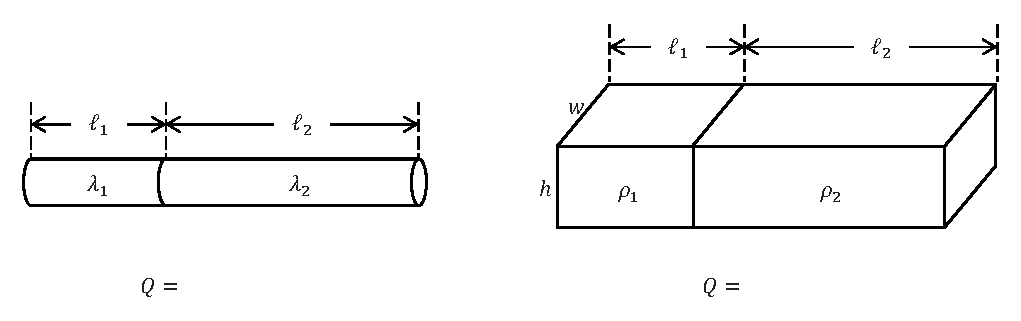
\includegraphics[width=0.75\textwidth]{charge_density/fig1.eps}
\end{center}

\item In general, if there are lots of bits o' charge $\Delta Q$, then the total charge is given by their sum, $Q = \sum_i \Delta Q_i$. For the thin rod, you just used $\Delta Q_i = \lambda_i \Delta x$.  For the rectangular bar in the figure below, express the bit o' charge $\Delta Q_i$ in terms of the quantities given in the picture: $h$, $w$, $\Delta x$ and $\rho_i$

\vspace{-0.4 in}
\begin{center}
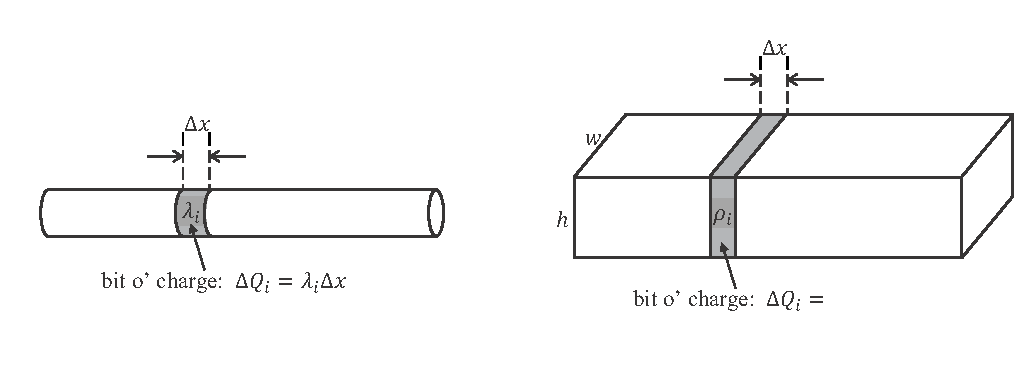
\includegraphics[width=0.75\textwidth]{charge_density/fig2.eps}
\vspace{-0.2in}
\end{center}
What if, instead of a finite number of uniform charge densities, the charge distribution on your object varies continuously, forming a smooth gradient. Instead of a discrete set of $\lambda_i$, your charge density would be some continuous function of position like $\lambda(x)$.  (That is, lambda as a function of $x$, not lambda times $x$.) No problem! Just imagine your finite $\Delta Q$ shrinking to an infinitesimal $dQ$.  For the thin rod, instead of $Q= \sum_i \Delta Q_i = \sum \lambda_i \Delta x$, you would use $Q = \int dQ = \int\lambda\left(x\right) dx$. 

\vspace{-0.1in}
\begin{minipage}{0.54\textwidth}
\item In the picture to the right, suppose $\lambda = Cx$, where $C$ is some constant. Write the integral to find the total charge $Q$ of the rod, starting with $Q = \int dQ$, including the limits of integration.  Evaluate the integral to get $Q$.
\end{minipage}
\begin{minipage}{0.45\textwidth}
    \hspace{0.25in}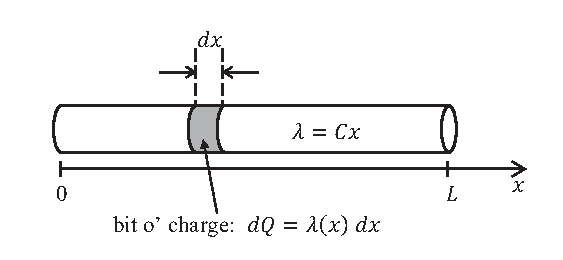
\includegraphics[width=0.9\textwidth]{charge_density/fig3.eps}
\end{minipage}
\answerspace{0.4 in}


\pagebreak[2]

In the picture below, suppose $\rho = Cx^2$, where $C$ is some constant. To find the total charge $Q$, you will again use $Q = \int dQ$, but this time you'll write $dQ = \rho \,dV$.  
\vspace{-0.2 in}
\begin{center}
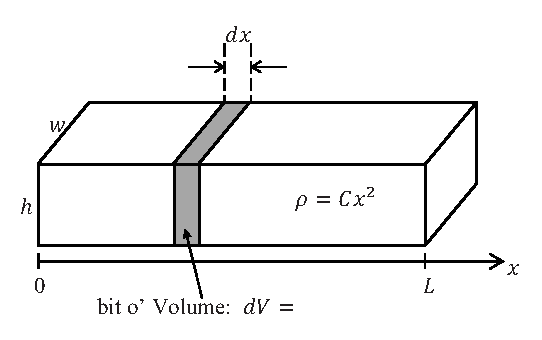
\includegraphics[width=0.40\textwidth]{charge_density/fig4.eps}
\end{center}

\item What is $dV$, in terms of quantities given in the picture?
\vspace{0.3in}

\item Write the integral, with limits, to find the total charge $Q$ of the block.  Evaluate the integral to get $Q$.
\vspace{1.0in}

Finally, we'll consider a solid cylinder of charge with height $h$ and radius $R$, where the charge density varies as $\rho = Cr$.  Again, we'll find the total charge by setting up an integral. 

For the rectangular block, we cut it into slices along the $x$ axis, so that each slice only had one value of $\rho$.  To cut the cylinder so that each slice has only one value of $\rho$, we'll have to cut it into concentric rings of radius $r$ like the picture below, then imagine unrolling each ring into a thin rectangular sheet.

\begin{center}
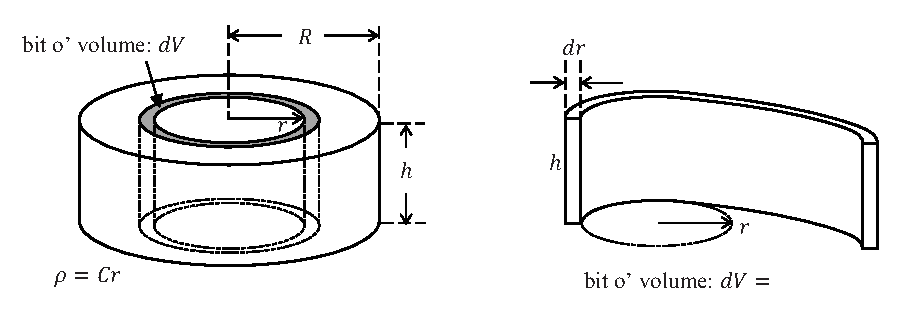
\includegraphics[width=0.85\textwidth]{charge_density/cylinders.eps}
\end{center}

\item What is the volume $dV$ of the thin rectangular sheet, expressed in terms of the quantities given in the picture above?
\vspace{0.3in}

\item Find the charge $Q$ of the cylinder by evaluating an integral over $dr$, starting with $Q = \int dQ$.  What are the limits of integration? 
\end{enumerate}


